% This is "sig-alternate.tex" V2.0 May 2012
% This file should be compiled with V2.5 of "sig-alternate.cls" May 2012
%
% This example file demonstrates the use of the 'sig-alternate.cls'
% V2.5 LaTeX2e document class file. It is for those submitting
% articles to ACM Conference Proceedings WHO DO NOT WISH TO
% STRICTLY ADHERE TO THE SIGS (PUBS-BOARD-ENDORSED) STYLE.
% The 'sig-alternate.cls' file will produce a similar-looking,
% albeit, 'tighter' paper resulting in, invariably, fewer pages.
%
% ----------------------------------------------------------------------------------------------------------------
% This .tex file (and associated .cls V2.5) produces:
%       1) The Permission Statement
%       2) The Conference (location) Info information
%       3) The Copyright Line with ACM data
%       4) NO page numbers
%
% as against the acm_proc_article-sp.cls file which
% DOES NOT produce 1) thru' 3) above.
%
% Using 'sig-alternate.cls' you have control, however, from within
% the source .tex file, over both the CopyrightYear
% (defaulted to 200X) and the ACM Copyright Data
% (defaulted to X-XXXXX-XX-X/XX/XX).
% e.g.
% \CopyrightYear{2007} will cause 2007 to appear in the copyright line.
% \crdata{0-12345-67-8/90/12} will cause 0-12345-67-8/90/12 to appear in the copyright line.
%
% ---------------------------------------------------------------------------------------------------------------
% This .tex source is an example which *does* use
% the .bib file (from which the .bbl file % is produced).
% REMEMBER HOWEVER: After having produced the .bbl file,
% and prior to final submission, you *NEED* to 'insert'
% your .bbl file into your source .tex file so as to provide
% ONE 'self-contained' source file.
%
% ================= IF YOU HAVE QUESTIONS =======================
% Questions regarding the SIGS styles, SIGS policies and
% procedures, Conferences etc. should be sent to
% Adrienne Griscti (griscti@acm.org)
%
% Technical questions _only_ to
% Gerald Murray (murray@hq.acm.org)
% ===============================================================
%
% For tracking purposes - this is V2.0 - May 2012

\documentclass{sig-alternate}
\usepackage{graphicx}
\begin{document}
%
% --- Author Metadata here ---
\conferenceinfo{WOODSTOCK}{'97 El Paso, Texas USA}
%\CopyrightYear{2007} % Allows default copyright year (20XX) to be over-ridden - IF NEED BE.
%\crdata{0-12345-67-8/90/01}  % Allows default copyright data (0-89791-88-6/97/05) to be over-ridden - IF NEED BE.
% --- End of Author Metadata ---
\title{Godzilla: A Cloud Key-Value storage with Replication, Failure Detection and Notification}%\titlenote{(Produces the permission block, and
%copyright information). For use with
%SIG-ALTERNATE.CLS. Supported by ACM.}}
%\subtitle{[Extended Abstract]
%\titlenote{A full version of this paper is available as
%\textit{Author's Guide to Preparing ACM SIG Proceedings Using
%\LaTeX$2_\epsilon$\ and BibTeX} at
%\texttt{www.acm.org/eaddress.htm}}}
%
% You need the command \numberofauthors to handle the 'placement
% and alignment' of the authors beneath the title.
%
% For aesthetic reasons, we recommend 'three authors at a time'
% i.e. three 'name/affiliation blocks' be placed beneath the title.
%
% NOTE: You are NOT restricted in how many 'rows' of
% "name/affiliations" may appear. We just ask that you restrict
% the number of 'columns' to three.
%
% Because of the available 'opening page real-estate'
% we ask you to refrain from putting more than six authors
% (two rows with three columns) beneath the article title.
% More than six makes the first-page appear very cluttered indeed.
%
% Use the \alignauthor commands to handle the names
% and affiliations for an 'aesthetic maximum' of six authors.
% Add names, affiliations, addresses for
% the seventh etc. author(s) as the argument for the
% \additionalauthors command.
% These 'additional authors' will be output/set for you
% without further effort on your part as the last section in
% the body of your article BEFORE References or any Appendices.

\numberofauthors{2} %  in this sample file, there are a *total*
% of EIGHT authors. SIX appear on the 'first-page' (for formatting
% reasons) and the remaining two appear in the \additionalauthors section.
%
\author{
% You can go ahead and credit any number of authors here,
% e.g. one 'row of three' or two rows (consisting of one row of three
% and a second row of one, two or three).
%
% The command \alignauthor (no curly braces needed) should
% precede each author name, affiliation/snail-mail address and
% e-mail address. Additionally, tag each line of
% affiliation/address with \affaddr, and tag the
% e-mail address with \email.
%
% 1st. author
\alignauthor
Mohsen Ahmadvand
			%\titlenote{Dr.~Trovato insisted his name be first.}\\
       %\affaddr{Institute for Clarity in Documentation}\\
       %\affaddr{1932 Wallamaloo Lane}\\
       %\affaddr{Wallamaloo, New Zealand}\\
       \email{mohsen.ahmadvand@tum.de}
% 2nd. author
\alignauthor
Ibrahim AlZant
%\titlenote{The secretary disavows
%any knowledge of this author's actions.}\\
       %\affaddr{Institute for Clarity in Documentation}\\
       %\affaddr{P.O. Box 1212}\\
       %\affaddr{Dublin, Ohio 43017-6221}\\
       \email{ibrahim.alzant@tum.de}
% 3rd. author
\and
\alignauthor 
Arash Khatayee
%Lars Th{\o}rv{\"a}ld\titlenote{This author is the
%one who did all the really hard work.}\\
       %\affaddr{The Th{\o}rv{\"a}ld Group}\\
       %\affaddr{1 Th{\o}rv{\"a}ld Circle}\\
       %\affaddr{Hekla, Iceland}\\
       \email{arash.khatayee@tum.de}
%\and  % use '\and' if you need 'another row' of author names
%% 4th. author
%\alignauthor Lawrence P. Leipuner\\
       %\affaddr{Brookhaven Laboratories}\\
       %\affaddr{Brookhaven National Lab}\\
       %\affaddr{P.O. Box 5000}\\
       %\email{lleipuner@researchlabs.org}
%% 5th. author
%\alignauthor Sean Fogarty\\
       %\affaddr{NASA Ames Research Center}\\
       %\affaddr{Moffett Field}\\
       %\affaddr{California 94035}\\
       %\email{fogartys@amesres.org}
%% 6th. author
%\alignauthor Charles Palmer\\
       %\affaddr{Palmer Research Laboratories}\\
       %\affaddr{8600 Datapoint Drive}\\
       %\affaddr{San Antonio, Texas 78229}\\
       %\email{cpalmer@prl.com}
}
% There's nothing stopping you putting the seventh, eighth, etc.
% author on the opening page (as the 'third row') but we ask,
% for aesthetic reasons that you place these 'additional authors'
% in the \additional authors block, viz.
%\additionalauthors{Additional authors: John Smith (The Th{\o}rv{\"a}ld Group,
%email: {\texttt{jsmith@affiliation.org}}) and Julius P.~Kumquat
%(The Kumquat Consortium, email: {\texttt{jpkumquat@consortium.net}}).}
\date{22 January 2015}
% Just remember to make sure that the TOTAL number of authors
% is the number that will appear on the first page PLUS the
% number that will appear in the \additionalauthors section.

\maketitle
\begin{abstract}
Key value store is at the core of many large scale distributed services to handle petabytes of data across thousands of servers and network components located in many datacenters around the world. At this scale, many components may fail continuously. In order to keep these systems functional, reliability, availability, scalability and persistent state infrastructures are required. 

This paper presents the design and implementation of a key value store, which is highly available and reliable in terms of persistent state, and also provides the scalability capability. To achieve scalability a similar approach to chord implementation of DHT is used. Availability and reliability are provided using a replication strategy alongside a low over head failure detection system. Whenever a node is failed, its data is recovered using its replica servers, so persistent state is guaranteed and the probability of loss of data is very low.
%This paper provides a sample of a \LaTeX\ document which conforms,
%somewhat loosely, to the formatting guidelines for
%ACM SIG Proceedings. It is an {\em alternate} style which produces
%a {\em tighter-looking} paper and was designed in response to
%concerns expressed, by authors, over page-budgets.
%It complements the document \textit{Author's (Alternate) Guide to
%Preparing ACM SIG Proceedings Using \LaTeX$2_\epsilon$\ and Bib\TeX}.
%This source file has been written with the intention of being
%compiled under \LaTeX$2_\epsilon$\ and BibTeX.
%
%The developers have tried to include every imaginable sort
%of ``bells and whistles", such as a subtitle, footnotes on
%title, subtitle and authors, as well as in the text, and
%every optional component (e.g. Acknowledgments, Additional
%Authors, Appendices), not to mention examples of
%equations, theorems, tables and figures.
%
%To make best use of this sample document, run it through \LaTeX\
%and BibTeX, and compare this source code with the printed
%output produced by the dvi file. A compiled PDF version
%is available on the web page to help you with the
%`look and feel'.
\end{abstract}

%% A category with the (minimum) three required fields
%\category{H.4}{Information Systems Applications}{Miscellaneous}
%%A category including the fourth, optional field follows...
%\category{D.2.8}{Software Engineering}{Metrics}[complexity measures, performance measures]
%
%\terms{Theory}

\keywords{Failure detection, Key-Value Storage, Cloud}

\section{Introduction}

In the past, one server was enough to serve thousands of clients. This server was separating data layer from the application layer by delegating data retrieval to a sql server to improve efficiency and transparency. With the growth of Internet technologies and huge increase in number of users and amount of data stored and requested, new requirements have been arose, which could not be provided by typical client server architecture. These requirements were consisting of highly demanded scalability, reliability, consistency and minimum latency. Moving to Cloud environment was a solution to these requirements and problems. In order to provide these requirements, some problems need to be taken into account such as dealing with failures, keeping data consistent, and preventing the loss of data.%failure detection %replication.
Over a decade of research in cloud computing effective solutions has been achieved aiming to satisfy mentioned properties using a peer to peer communication concepts between a group of server nodes. 

%These nodes build up a key value store to leverage cloud scalability and reliability. Key value storages are being used by many data exhaustive applications such as Facebook, YouTube and Google Drive.  

%Nowadays, the need for efficient and reliable big data storages has significantly increased.
Massive user requests, massive amount of data, and dealing with failures are main motivations to move to the cloud storages. Although relational databases are good solution in dealing with structured data and can respond to complicated queries, by design they are not easly scalable, so they cannot be used effectively in cloud environment. Furthermore, faster response is required which is not achievable with relational databases in communication with huge number of users. Instead cloud databases deal with data as pairs of key and value which is known as NoSQL database. In key-value stores there is no consistent structure defined for data. Thus, NoSQL databases are fast, highly scalable, replicable, and can deal with variable structured data. Key value storages are being used by many data exhaustive applications such as Facebook, YouTube and Google Drive
%On the same hand, the usage of software programs such as Facebook, YouTube and blogs has accelerated in forms of mobile applications as well as web applications. 

Key value store can be used rigorously by all application developers who are seeking for highly scalable and reliable data storages. Use cases of  these kind data stores could be as following, online stores, e-commerces, video sharing, social media applications, electronic votings, hotel booking, travel agency and etc. We insist that, usage of the key value storages is not limited to the mentioned use cases and any massive user targeted solution can be potential candidate.

In this paper we have implemented and evaluated a highly scalable and reliable  key value storage using state of the arts literature and  techniques in the field supplied to us during our practical training course. 

The rest of this paper is structured as following Section 2 Related work, discusses the related literature in the field and their applicability to our implementation. Section 3 Approach presents the design decisions that we have made in our system. Plus to that, we present the extension component to our key value store in Section 3. Latter, we have evaluated our solution and experimented our application aiming to study performance of our key value store.  Finally, in the last section Conclusion, we have explained the our evaluation results.

%The \textit{proceedings} are the records of a conference.
%ACM seeks to give these conference by-products a uniform,
%high-quality appearance.  To do this, ACM has some rigid
%requirements for the format of the proceedings documents: there
%is a specified format (balanced  double columns), a specified
%set of fonts (Arial or Helvetica and Times Roman) in
%certain specified sizes (for instance, 9 point for body copy),
%a specified live area (18 $\times$ 23.5 cm [7" $\times$ 9.25"]) centered on
%the page, specified size of margins (1.9 cm [0.75"]) top, (2.54 cm [1"]) bottom
%and (1.9 cm [.75"]) left and right; specified column width
%(8.45 cm [3.33"]) and gutter size (.83 cm [.33"]).
%
%The good news is, with only a handful of manual
%settings\footnote{Two of these, the {\texttt{\char'134 numberofauthors}}
%and {\texttt{\char'134 alignauthor}} commands, you have
%already used; another, {\texttt{\char'134 balancecolumns}}, will
%be used in your very last run of \LaTeX\ to ensure
%balanced column heights on the last page.}, the \LaTeX\ document
%class file handles all of this for you.
%
%The remainder of this document is concerned with showing, in
%the context of an ``actual'' document, the \LaTeX\ commands
%specifically available for denoting the structure of a
%proceedings paper, rather than with giving rigorous descriptions
%or explanations of such commands.
\section{Related Works}
David Karger et al., 1999 \cite{consistentHashing} in their research work have presented the idea of web caching with the use of consistent hashing technique. They have shown that using consistent hashing load  balance and fault tolerance is handled much efficient. 
In this work we have used consistent hashing for mapping keys to server nodes, such that adding and removing nodes ensures a balanced load.

A few years later, the need for an efficient way to locate nodes in a distributed peer to peer network motivated Ion Stoica et al., 2002 \cite{chord} to came up with the chord protocol. In their protocol, for a given key, it is easily computable to find the responsible server. This has been done with leveraging consistent hashing technique along with a novel finger table per each node. Such that, each node by referring to its own finger table can route the key to mapping server. They have shown average lookup time for N nodes for a given key is (1/2) Log N. 

Dong Dai et al., 2012 \cite{memory} explained that keeping cloud data storages in the memory rather than disks improves the retrieval and decreases the latency in key value storages. Therefore, we cashing most recent key-value pairs in the RAM to improve the latency in our system.

Beside these literatures which targeted the scalability of the system, in \cite{heartbeat} a method for failure detection using heartbeats has been introduced. In their method, failure detection is not based on the timeout  but an agreement on failure has been taken into account. Their method is applicable in case of message losses or process failures.


\section{Approach}
\subsection{Design Decisions}
Our key-value storage is consist of three subsystems as Client, Server and External Configuration Service. These subsystems are descibed in details in the section \ref{implementation}. In this section, we explained our design decisions that effected all subsystems namely  \textbf{Replication}, \textbf{Failure detection} and the final \textbf{Extension} that we have added to the system. 

\subsubsection{Replication}
Reliability and consistency are two of the most important factors in designing scalable web services running on cloud environments. With integrating replication into our system we achieved to overcome the loss of data, omitted the problem of single point of failure, and reduced the load on the servers. The strategy was to store each server's data also as replicated data on two other servers. Whenever a server crashes or is not available, the data can be recovered from these replicas, and the probability of the loss of the data is  significantly decreased. The replica servers will also respond to clients' GET requests, so the load on each server is distributed between two other replica servers. 

In order to implement replication with gradual consistency we designed our meta data in a way that each server will recognize its own replicas and coordinators. Each updates of the data by a client (PUT, DELETE) will directly go to the main responsible server, called Coordinator. Then the coordinator will sends these updates as replication to the two next nodes in the clockwise direction in ring topology, known as replicas. Each Server has 3 persistent storage, one for storing the key value pairs which currently this server is responsible for, and two other storages to store replicated data from its coordinators. During the start up of the system after the ECS has calculated the meta data, and all the roles in the system has been assigned, the replication operation starts. During this operation the ECS will command each sever to send the portion of the data in its main persistent storage that currently (in this topology) is owned by this server for replication to its replicas.  

In the scenario of the GET request, each server will also respond to the client, if it has the Key either in is own main storage or as replicated data from of its coordinators. However, to increase consistency if the key is in one of his coordinators' range and no value is mapped to this key, the server will respond with \textbf{SERVER NOT RESPONSIBLE} and a meta data update, so the client would contact the main server. Thus, it is possible for a client to get an old value for a key in the system, but never a client would get a null value if there is already a value mapped to the respected key in the system.

During the add or removal of a node the ECS will inform the affected servers, so alongside the data which has to be moved between the servers because of the change in responsibility of that data, the data for replication is also moved. Thus, each new state of the system is also consistent with respect to replication. In case of detection of a failed node, the replication storage of the successor of that node is used to recover the lost data. 
\subsubsection{Failure Detection}
Our failure detection is based on replica failure reports. Coordinatore nodes 
constantly send heartbeat messages to its replica list. Each replica by looking at the metadata knows its coordinator node. These replicas have been equipped with an internal timeout thread which is currently set to 3 minutes. On the other side, the coordinator in 10 second intervals sends a very small sized heartbeat package to the replica list. As soon as this message being received by the replica  it will reset the timeout thread. In case that the replica does not receive the heartbeat message from the coordinator before the defined timeout, it will trigger the failure   detected method on replica side. Thus the replica sends a failure detected message along with his own id and failed coordinator id to the ECS. 
ECS considers a failure in a server only in case of agreement as described in follows. ECS first ensures the uniqueness and freshness of a failure message. Uniqueness refers to reporter id in which one given replica can only vote once for a failure. Samwise, freshness refers to the time that the failure message has been received. ECS ignores the failure reports with old timestamps.
In the figure \ref{failuredetection} the failure detection sketch has been illustrated.


\begin{center}
\begin{figure}[ht!]
\centering
     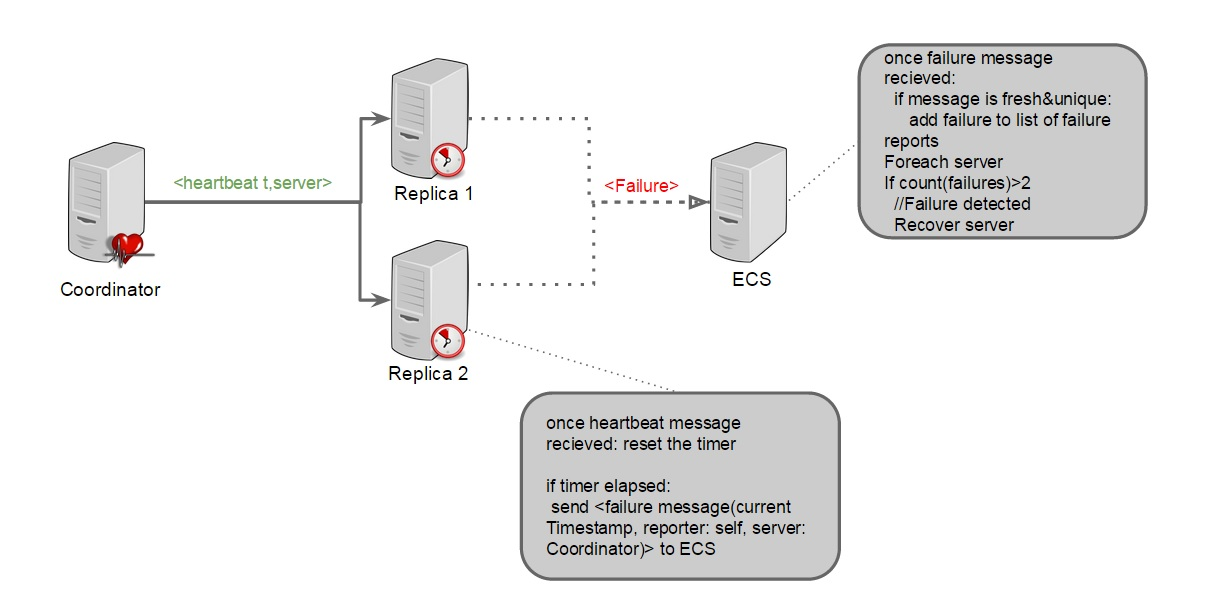
\includegraphics[width=0.5\textwidth]{FailureDetection.jpg}
\caption{Failure Detection Sketch \label{failuredetection}}
\end{figure}
\end{center}

\subsection{Extension: Subscription/Notification System }
%\subsubsection{}

We provided data subscription capability as an extension to our key value store system. By implementing  this functionality, a client is able to keep track of the data which is important to him and get the newest value, whenever a change has been occurred. 

The subscribed key value pairs are stored on a cache on the client side alongside a hash list of subscribed servers and keys. This cache is used to respond to handle GET requests of subscribed keys. As a result the load on the network and the servers will be reduced. Furthermore, this cache is guaranteed to provide the recent value of a key until the responsible server of that key has been changed, due to an addition or removal of a node. When the new meta data has reached to the client, the client will resubscribe to all the previously subscribed keys, which their responsible server have been changed, and the cache is fully reliable again. By making clients responsible for keeping their subscriptions consistent, there is no overhead on the server side regarding this issue.

On the server side the list of subscribed keys and the clients who are interested in getting notifications about their value is being kept. In case of any changes to the value, every subscribed client will get notified with the recent value. These information is kept in memory in servers in order to have a fast access to data and more efficiency. Thus, in case of removal or failure of a node these information will be lost on the server side, but as it was mentioned the client will always keep its subscription list updated whenever he recognizes any change in the system formation.


\section{Implementation}\label{implementation}
Key-value storage consists of three subsystems namely KVClient, KVServer, KVECS. 
In this section we descibe each subsystem in details. However, full source codes are available on Github accessible at \cite{github}. 
\subsection{Client}
KVClient is the user intermediate layer in which the end-user with knowing only one server location can start using the cloud storage. KVClient application has following main features: \\
\textbf{CONNECT} which allows the user to establish a connection to a server\\
\textbf{PUT} let user to store a key value pair in a server. In case that server is not responsible for demanded key the switching to the responsible server has been done automatically to ensure better user experience.\\
\textbf{GET} user can query a key and like put command the responsibility of the servers has been encapsulated.\\
\textbf{GETS} it retrieves the queried key by the user similar to get command. Plus to that, the client will be notified about the queried  key changes. In other words, by using this command user will be subscribed to the corresponding server. Therefore, Any value changes of the key by any client will lead to a push notification to the subscribed client.\\
\textbf{PUTS} It stores a key-value pair and subscribe to the key changes just like the gets.\\
\subsubsection{Subscription on client side}
For the subscription part we have implemented a separate thread to keep listening to the notification messages from the responsible servers. Whenever a client wants to subscribe for a key, the port which this client is listening to get notifications is also send to the servers, so servers can identify the clients (Using Ip and this port) and contact them in case of sending notification. %In case that new servers being added or removed from the system, the responsible server for each key might change due to the mapping constraints in the ring. To deal with responsibility changes, upon metadata updates on client side we subscribe all keys to corresponding servers. By this approach eventual consistency is guaranteed as well as no overhead on server side because clients are keeping track of their subscription.\\ 
%On the server side, a list of subscribed servers per each key is being maintained and upon each put command the notifications are being published. For further details about the subscription feature refer to the server implementation details section \ref{serverimpl}.

\subsection{Server}\label{serverimpl}
KVServer is the main component in the server side. The KVServer is starting a new thread for each new client request. This new thread will handle any request come from clients including all client available operations.
In the same context, the server component includes a database manager component. This manager is responsible of storing and retrieving data in pairs from and into the server database. The database manager is a thread safe, supporting multiple threads accessing the data and perform different operation simultaneously. 

On other hand, the server side had multiple statuses. The reply from the server to client includes this status. The statuses of the server side are :\\
\textbf{UNDER INITIALIZATION}: This status represents that the server has not started to serve client yet and its under initialization operation from the ECS component.\\
\textbf{STOPPED}: In case of the server is stopped and not serving clients temporarily.\\
\textbf{SERVER WRITE LOCK}: This status means that the server is currently moving or receiving data from or to other servers.\\
\textbf{SERVER NOT RESPONSIBLE}: This status indicates that the requested data is not located on this server and also not replicated on this server. In case of this status, the server will send a copy of metadata to the client so it can redirect the request to the responsible server.\\
\textbf{GET ERROR, GET SUCCESS, GETS SUCCESS}: Indicates the status of the requested GET operation.\\
\textbf{PUT SUCCESS, PUTS SUCCESS, PUT UPDATE, PUT ERROR}: Indicates the status of the requested PUT operation.\\
\textbf{DELETE SUCCESS, DELETE ERROR}: Indicates the status of the requested PUT with null value - Delete- operation.

Additionally,The server component is responsible for serving the subscribe requests from the client side. It stores all clients information that interested in a specific pair, then it will notify all the subscribers in case of any change for this pair. see section 3.1.1.

Finally, Each instance of the server component is replicating the data into two other instances. At the same time it acts as a replica for other two server instances. see section 3.1.2. Moreover, each instance sends heartbeat to its replica instances in order to detect the failure of a node. see section 3.2

\subsection{External Configuration Service}
ECS is the component in our system, which coordinates KVServers, knows how the data is distributed in the system, and modifies this distribution whenever it is needed, such as when a node is added, removed, or failed. The ECS calculates the meta data and assigns key ranges to the servers. ECS's role in this system is comparable to master's role in Google's Big Table key value store.\cite{bigTable}. Furthermore, ECS has a User Interface to interact with the admin. Adding and removing a node(\textbf{add, remove}), starting and stopping the system(\textbf{start, stop}), and shutting down the system (\textbf{shutDown}) are the commands available for the admin of the system.

ECS will be started from a configuration file consisting of the list (IP,Port) of the servers called server's repository. Before the beginning of the cloud system or adding a new node to the system, ECS will try to run and start the required number of the servers from this repository list with  remote procedure calls made through SSH to the remote machines hosting the servers. 

During the add and remove operation, ECS will coordinate the affected servers to move their data, either for reassigning them (in case of add a new node) or for saving them as replication, to another servers. ECS will keep track of data movement operations, so whenever one of these move data operations failed and caused the system to lose some portion of data or put the system in an unstable state the ECS will undo the operation and will return the system back to the previous state before the add  or removal operation. However, if everything went as planned ECS will send the new meta data to the other servers, the ones which were not affected during these operations, so did not know about the current changes of the system till now.

In order to get the failure reports from the servers, the ECS has a server inside which is listening to a special port, 50018. This port is send to the servers during their initializations by ECS. Whenever a failure of a node has been dicovered (see section 3.1.2) %report comes in from any server, ECS will check to see if this report is valid. A report is valid if the reporter reports the failure of one of his coordinators. After validation was true ECS will increment the counter of failed reports for the suspected server. Furthermore, if there was already a failure report from the other replica of the respected failed server, ECS will set the counter to 0 and 
ECS will start the recovery operation. In recovery operation a new meta data is calculated, and ECS will command the successor of the failed server to recover the data of the failed server from its replication storage. Later on the affected servers will send replication data to their new replicas, and get replicated data from their new coordinators. At last, ECS will try to add a new node to the system.

\section{Evaluation}
\subsection{Dataset}
Data for our experiment, key value pairs, were gathered from the UNIX dictionary of British-English words. A large data set consisting of approximately one hundred thousand of words.
\subsection{Test prepration}
Before each test we populate 80 percent of data, key values, to our servers with respect to the current distribution of servers and their hash values in the ring topology. These data are stored in the main storage for each responsible server of that key, and in replicated storages of the replicas of that servers in ring topology. In order to simulate a real environment, where not only clients send request for keys already stored in the system, but also they will provide new key value pairs to the system. We designed our test clients to choose keys for their requests randomly from the same dataset. Thus, with 20 percent of chance they may choose a new key which is not still in the system and with 80 percent a key already stored in the system. 

\subsection{Test parameters}
The test plan was designed using Jmeter to measure the system performance under different parameters. The common setting for all test cases were:
\begin{enumerate}
\item Number of users that has been set to 1000
\item Ramp-up time that has been set to 20, which means 1/20 of total number of users, in this case 50, per second are being added to the system.
\item The main testing variable in each test was the number of launched KV servers.
\end{enumerate}
		
\subsection{Test Steps}								 			
1-  Setup test environment by launching ECS with requested number of servers by the test definition.\newline
2-  Executing parallel write operations simulating different users. The key-value pair are randomly retrieved from the test dataset as stated before.\newline
3-  Executing concurrent read operations of a random key retrieved from the test dataset. As only 80\% of the keys are available in the cloud storage, there is 20\% chance of requesting a key which does not exist on the servers and this will result to error(GET ERROR).\newline
4-  Shutting down ECS.	
			 					
\subsubsection{Test Environment}			
The test was conducted deploying all the components on the same machine, the test machine capabilities: Processor: Intel Core i5 CPU @ 2,4 GHz (4 CPUs) , Memory: 8 GB 1600 MHz DDR3

\subsection{Tests and Results}
\subsubsection{Test case1: ( 1000 clients, 1 server, 20 s ramp-up time)}
%Table to be added
\textbf{Write operation}:  Table \ref{put_1_1000_tbl} presents the performance results and figure \ref{put_1_1000} illustrates the response time graph for this  test case.
\begin{table}[h]
\begin{tabular}{|l|l|l|l|l|l|l|}
\hline
 \textbf{avg} & \textbf{med} & \textbf{min} & \textbf{max} & \textbf{error} & \textbf{Throughput/sec} \\ \hline
 97661 & 106326 & 309 & 366 & 0 & 4.77 \\ \hline
\end{tabular}\caption{Write operation measures(1000 clients, 1 server)}\label{put_1_1000_tbl}
\end{table}
\begin{center}
\begin{figure}[ht!]
     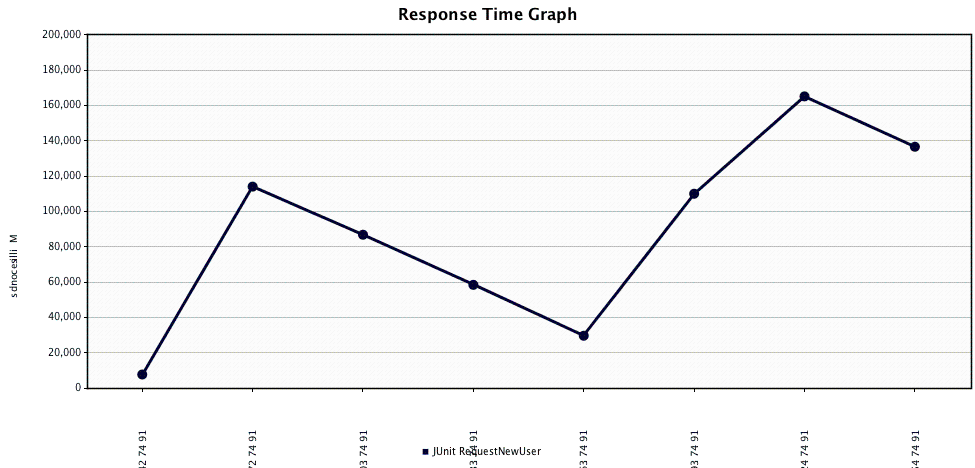
\includegraphics[width=0.5\textwidth]{put_1_1000_response.png}
\caption{Write operation (1000 clients, 1 server) \label{put_1_1000}}
\end{figure}
\end{center}
\textbf{Read operation}: Measures results shown in table \ref{get_1_1000_tbl}. The response time graph for the get requests has been shown in figure \ref{get_1_1000}.
\begin{table}[h]
\begin{tabular}{|l|l|l|l|l|l|}
\hline
\textbf{avg} & \textbf{med} & \textbf{min} & \textbf{max} & \textbf{error} & \textbf{Throughput/sec} \\ \hline
13 & 7 & 2 & 381 & 0.002 & 43.36 \\ \hline
\end{tabular}\caption{Read operation measures (1000 clients, 1 server)}\label{get_1_1000_tbl}
\end{table}
\begin{center}
\begin{figure}[ht!]
\centering
     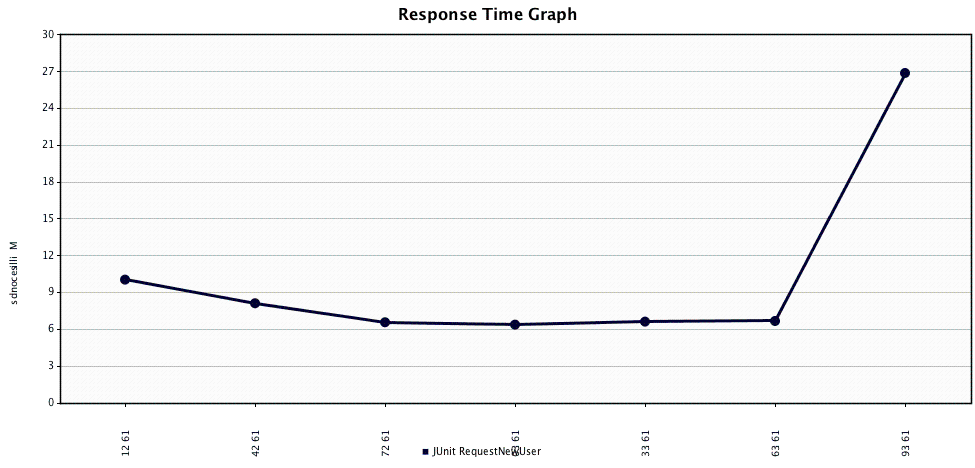
\includegraphics[width=0.5\textwidth]{get_1_1000_response.png}
\caption{Read operation (1000 clients, 1 server) \label{get_1_1000}}
\end{figure}
\end{center}
\subsubsection{Test case2: ( 1000 clients, 5 servers, 20 s ramp-up time)}
 \textbf{Write operation}: performance results shown in figure \ref{put_5_1000} and table \ref{put_5_1000_tbl}.
\begin{table}[h]
\begin{tabular}{|l|l|l|l|l|l|}
\hline
\textbf{avg} & \textbf{med} & \textbf{min} & \textbf{max} & \textbf{error} & \textbf{Throughput/sec} \\ \hline
20639 & 17827 & 40 & 56853 & 0 & 14.37029373 \\ \hline
\end{tabular}\caption{Write operation (1000 clients, 5 servers)}\label{put_5_1000_tbl}
\end{table} 
 \begin{center}
\begin{figure}[ht!]
\centering
     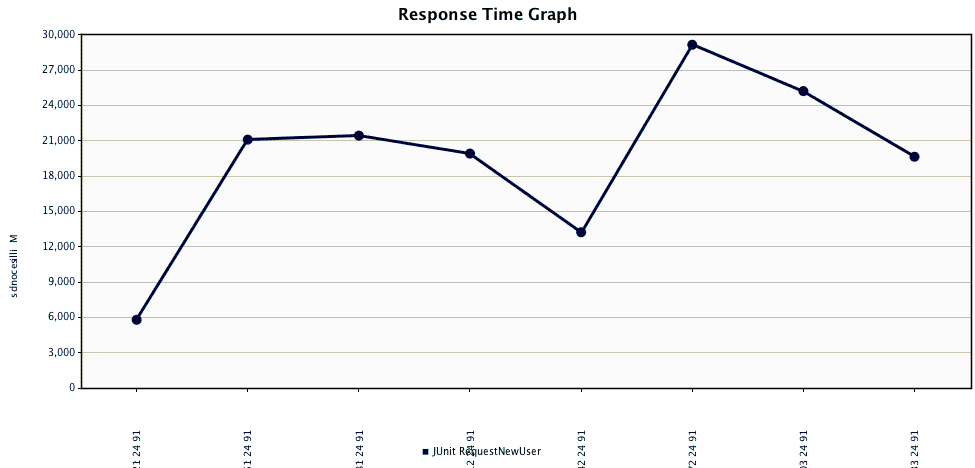
\includegraphics[width=0.5\textwidth]{put_5_1000_response.png}
\caption{Write operation (1000 clients, 5 servers) \label{put_5_1000}}
\end{figure}
\end{center}
 \textbf{Read opearation}: expermient results illustrated in figure \ref{get_5_1000} and table \ref{get_5_1000_tbl}.
 \begin{table}[h]
\begin{tabular}{|l|l|l|l|l|l|}
\hline
\textbf{avg} & \textbf{med} & \textbf{min} & \textbf{max} & \textbf{error} & \textbf{Throughput/sec} \\ \hline
55 & 12 & 2 & 1662 & 0.26 & 43.08487721 \\ \hline
\end{tabular}\caption{Read operation measures (1000 clients, 5 servers)}\label{get_5_1000_tbl}
\end{table}
 \begin{center}
\begin{figure}[ht!]
\centering
     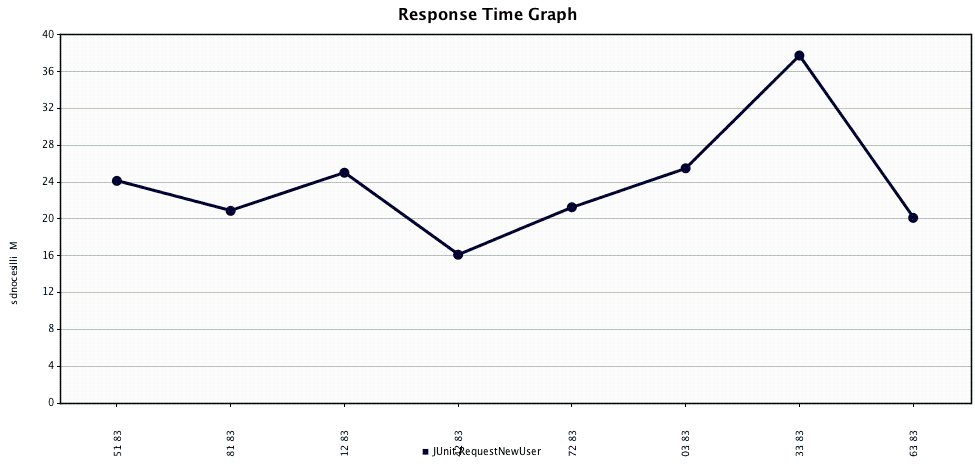
\includegraphics[width=0.5\textwidth]{get_5_1000_response.png}
\caption{Read operation (1000 clients, 5 servers) \label{get_5_1000}}
\end{figure}
\end{center}
\subsubsection{Test case3: ( 1000 clients, 10 servers, 20 s ramp-up time)}
 \textbf{Write operation}: operation experiment for this test case is shown in figure \ref{put_10_1000} and table \ref{put_10_1000_tbl}.
\begin{table}[h]
\begin{tabular}{|l|l|l|l|l|l|}
\hline
\textbf{avg} & \textbf{med} & \textbf{min} & \textbf{max} & \textbf{error} & \textbf{Throughput/sec} \\ \hline
9995 & 2600 & 9 & 50262 & 0 & 18.85298443 \\ \hline
\end{tabular}\caption{Write operation measures (1000 clients, 10 servers)}\label{put_10_1000_tbl}
\end{table} 
 \begin{center}
\begin{figure}[ht!]
\centering
     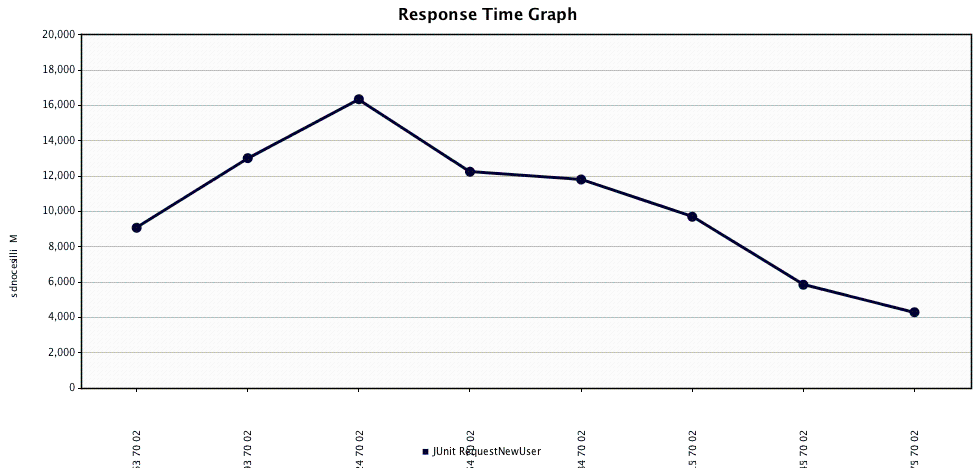
\includegraphics[width=0.5\textwidth]{put_10_1000_response.png}
\caption{Write operation (1000 clients, 10 servers) \label{put_10_1000}}
\end{figure}
\end{center}
 \textbf{Read operation}: requests performance results for this test case is presented in figure \ref{get_10_1000} and table \ref{get_10_1000_tbl}.
 \begin{table}[h]
\begin{tabular}{|l|l|l|l|l|l|}
\hline
\textbf{avg} & \textbf{med} & \textbf{min} & \textbf{max} & \textbf{error} & \textbf{Throughput/sec} \\ \hline
30 & 12 & 2 & 397 & 0.21 & 42.86877867 \\ \hline
\end{tabular}\caption{Read operation measures (1000 clients, 10 servers)}\label{get_10_1000_tbl}
\end{table}
 \begin{center}
\begin{figure}[ht!]
\centering
     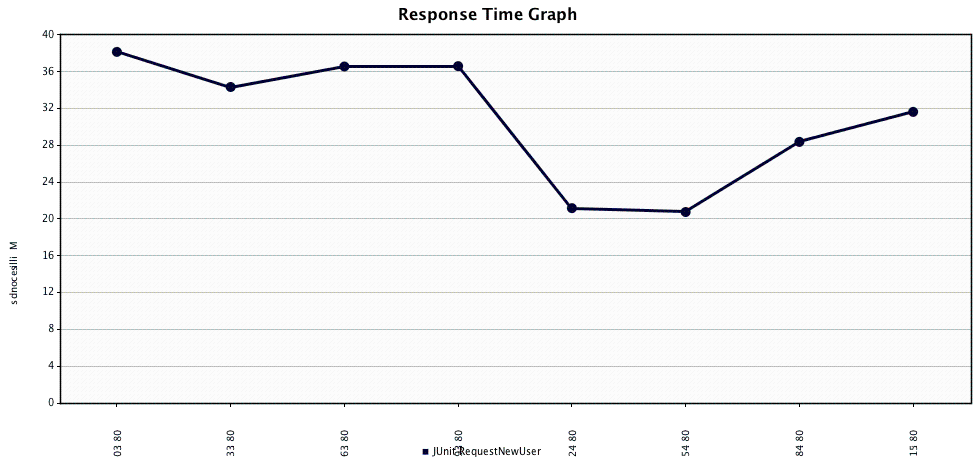
\includegraphics[width=0.5\textwidth]{get_10_1000_response.png}
\caption{Read operation (1000 clients, 10 servers) \label{get_10_1000}}
\end{figure}
\end{center}
\subsubsection{Test case4: ( 1000 clients, 10 servers, 20 s ramp-up time) without saving after each put request}
 \textbf{Write operation}: operations performance results without constantly saving to persistance storage after each request is presented in figure \ref{put_10_1000_nosave} and table \ref{put_10_1000_nosave_tbl}.
 \begin{table}[h]
\begin{tabular}{|l|l|l|l|l|l|}
\hline
\textbf{avg} & \textbf{Med} & \textbf{Min} & \textbf{max} & \textbf{error} & \textbf{Throughput/sec} \\ \hline
14 & 14 & 3 & 97 & 0.21 & 43.07188698 \\ \hline
\end{tabular}\caption{Write operation measures (1000 clients, 10 servers) no save after each operation}\label{put_10_1000_nosave_tbl}
\end{table}
 \begin{center}
\begin{figure}[ht!]
\centering
     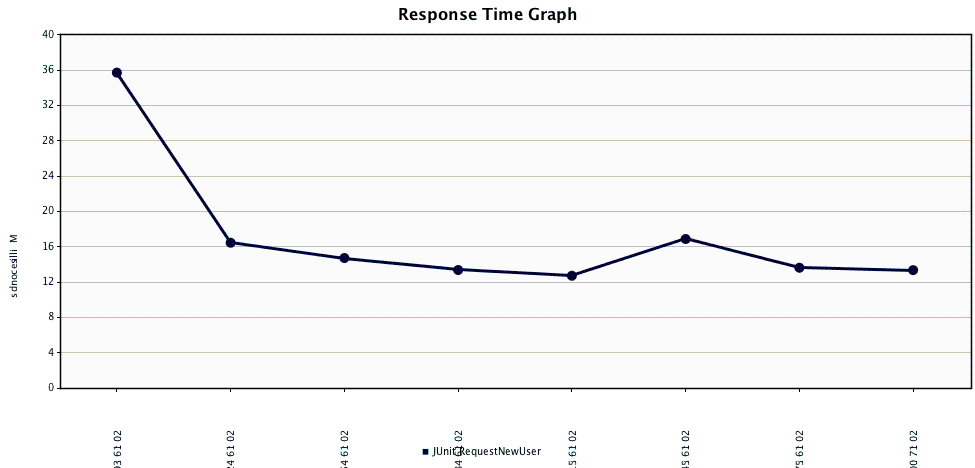
\includegraphics[width=0.5\textwidth]{put_10_1000_response_nosave.png}
\caption{Write operation (1000 clients, 10 servers) \label{put_10_1000_nosave}}
\end{figure}
\end{center}
 \textbf{Read operation}:
Not mentioned as it is the same as test case 3 read results. 
\section{Discussion}
This section is about discussing the results of the previous performance measurements. In the beginning, it is important to mention that the number of users (running threads) and ramp-up are fixed in all previous test cases. The only change is with the number of the servers, since those test cases aim to test the load balance between servers and its influence on the overall performance.

In the first test case, with only one server running, the graph for the read operation shows that the performance started with a good response times. By the end of the test case, the performance is getting slower and the response time increased. The reason behind this increasing in the response time is that the number of user threads is increasing 50 users per second since the ramp up time is 20.

On other hand, the graph of the write operations shows that the performance of write operations has some overhead. This overhead is due to the synchronization between threads in the writing operation, since the system is moving  the "in-memory" cache storage into the persistence storage after each write operation. 

By comparing the results from the second test case, which has five servers instead of one server, the read operations graph shows that the performance of the read operation is getting slower after increasing the number of servers. This leak of performance is due to switching the connection from one server to other by the client threads. The client threads are switching the connection based on the hash value for the inserted key. On other hand, the interesting point is that the performance of the write operation is improved five times comparing to the previous test case. The reason of this improvement is that the load has been balanced between five servers instead of only one server. In that case, the synchronization between threads for the write operation and moving the "in-memory" cache into persistence storage is distributed between servers which has the impact the performance of the write operations.

In the third test case, the number of the servers has increased up to 10 servers. Again, the performance of the read operations is getting slower since the users threads need to switch between ten servers instead of five. Although, comparing the results with the second test case results, the performance of the write operations has been improved twice.  This improvement  is a result of balancing the load into ten servers.

Eventually, the fourth test case is exactly the same as the third one, but without moving the "in-memory" cache into persistence storage after each write operation. Instead of that, moving the "in-memory" cache is moved into persistence storage only at the shutdown time. In that case, all the operations are done in the memory without performing any I/O operations. As a result of this change, the performance has been improved dramatically, since the user threads do not need to wait for persistence storage operations.
In conclusion for the previous results, the more servers the system has, the slower performance for the read operations. This leak of performance is due to the switching 
\section{Conclusion}
% serve clients from the in memory cache as much as possible,  avoid keeping clients waiting for persistency of the data.
We have provided a key value storage which is highly reliable in terms of data persistance state using replication mechanism. Beside that, a heartbeat system with minimum overheads while being able to detect actual failures has been introduced. Furthermore, we designed and implemented a publish-subscribe extention for our KV-Store which can be really handy for cloud based applications such as chatting and data storages.

According to our evaluation results, the more servers the system has, the slower performance for the read operations. This leak of performance is due to the switching between servers based on the hash value of the key. On other hand, the performance of the write operations is getting better since the synchronization between user threads is distributed among servers. In the same context, avoiding the persistence storage after each write operation and just performing that once at the shutdown time will improve the performance dramatically as seen in the last test case.

As future work of this project we propose, a mechanism to periodically persist the running cache and discover the trade off between increasing the cache size (to load key-value pairs into the memory) and latency of the servers. 

%ACKNOWLEDGMENTS are optional
\section{Acknowledgments}
We would like to acknowledge the support and guidance from the  Chair of Business Information Systems (Prof. Jacobsen) of Technische Universit{\"a}t M{\"u}nchen.
%
% The following two commands are all you need in the
% initial runs of your .tex file to
% produce the bibliography for the citations in your paper.
\bibliographystyle{abbrv}
\bibliography{sigproc}  % sigproc.bib is the name of the Bibliography in this case
% You must have a proper ".bib" file
%  and remember to run:
% latex bibtex latex latex
% to resolve all references
%
% ACM needs 'a single self-contained file'!
%
%APPENDICES are optional
%\balancecolumns

%\balancecolumns % GM June 2007
% That's all folks!
\end{document}
